\documentclass{article}
\usepackage[utf8]{inputenc}
\usepackage{parskip}
\setlength{\parindent}{0cm}
\usepackage{natbib}
\usepackage{graphicx}

\begin{document}

\title{An iOS Application for Snake Breed Identification and Object Detection Based on Deep Learning}
\author{Zhengyu Chen \\ The University of Melbourne \\ zhengyuc@student.unimelb.edu.au}
\date{Semester 1, 2019}
\maketitle
\newpage

\tableofcontents
\newpage

\section{Abstract}

Deep learning is


\section{Introduction}

\subsection{Deep Learning}

With the increment in the amount of data, deep learning performs much better on accuracy than traditional machine learning algorithms when, and deep neural networks have been a great approach to win numerous contests in machine learning and image recognition in recent years. Shallow and deep neural networks are distinguished by the depth of layers, which are chains of learnable links between actions and effects. Deep learning is inspired by human brains and how they perceive information through interactions of neurons. It’s a branch of machine learning and is implemented through large neural networks \cite{1}.

However, training deep neural networks is a difficult task. Firstly, it requires lots of labelled data as well as huge computing power. Secondly, classical methods that have proved effective when applied to shallow architectures are not as efficient when adapted to deep architectures. Thirdly, Adding layers does not necessarily lead to better solutions. The more the number of layers in a neural network, the lesser the impact of the back-propagation on the first layers \cite{2}. Because with such a deep neural network, if the gradients increase or decrease exponentially by the activation function, then these values could get really big or really small. And this makes training difficult, then gradient descent will take tiny little steps. It will take a long time for gradient descent to learn anything \cite{4}. Besides, the gradient descent tends to get stuck in local minima or plateaus \cite{3}. In fact, for a long time, this problem was a huge barrier to train deep neural networks. One partial solution is to choose a random initialization for the parameters of the neural network to make them have a mean of 0 and a standard variance of 1. It helps reduce the problem because it tries to set each of the weight matrices by not far from 1 to ensure it doesn't explode or vanish too quickly.

\subsubsection{Transfer Learning}

Neural network architectures that work well on some certain computer vision tasks often work well on other tasks due to the versatility of feature detectors. Sometimes the training process takes a few days or even more, and might require a lot of computing power. At this time, download the pre-trained models and use it as a start, which is called transfer learning, is a good initialization. 

Transfer learning is an effective way to make use of knowledge learned from the previous dataset to enhance a new model performance within the same domain \cite{day2017survey}. There are three possible benefits when using transfer learning. With transfer learning, we can have a high start, scope and asymptote, which shortens the training time and improves the outcome performance \cite{olivas2009handbook}. In order to do transfer learning, we only need to freeze most of the layers in the front to ensure the feature detector are preserved. Then remove the output layer and add a few hidden layers, and use our own softmax activation function to do the prediction. Since we have a relatively small dataset in this project, using transfer learning is an effective way to enhance performance.

\subsubsection{Overfitting}

Overfitting refers to that when a model fits the training data well but cannot predict the test data correctly, we may say that the model lacks the ability of generalization. When we observe that the accuracy on the training data has reached a very high ratio while the accuracy on the validation data still remains not high enough, or even a little bit low, and the value of loss function on the training data is much lower than that value on the validation data, we can say there is overfitting.

\begin{figure}[h]
\centering
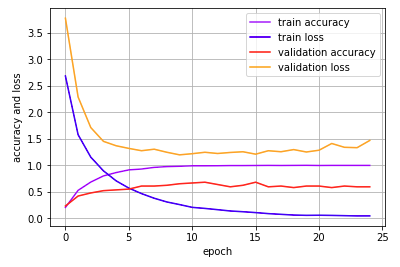
\includegraphics[scale=0.5]{Overfitting.png}
\caption{overfitting}
\label{fig:Overfitting.png}
\end{figure}

The most efficient way to prevent overfitting is to perform regularization on neural networks. Regularization constrains the learning process by adding a regularization term. In deep learning, there are two commonly-used regularization methods: Batch Normalization and Dropout.

Batch Normalization is proposed to solve two problems. One is that the input distribution of each layer changed as the number of layers deepens due to the activation functions. The other is that former layers need to adapt to the change of distribution. These two problems are called Internal Covariate Shift. We perform normalization on each layer separately, making the features of each layer have a mean of 0 and a variance of 1, which lets the value of each layer propagate in the effective range. we can also add a linear transformation operation so that the data can restore the ability of expression. Batch Normalization increases the robustness by normalizing the parameter. This constraint also improves the structural rationality of the system, and also accelerate convergence and prevent over-fitting.

Dropout means that when we are training the model, we can set a probability P for eliminating a node in the deep neural network. For each node, there is a probability of (1-P) for keeping it and a probability of P for dropping it. Then we perform forward-propagation and backpropagation-propagation on this much-diminished deep neural network. At each training step of a mini-batch dataset, the process of dropout creates a different deep neural network by randomly removing some units regarding the probability P. The process of dropout is similar to use ensemble learning on many different deep neural networks, each trained with a separate mini-batch dataset but share some context in the process of training. Since each classifier has been trained separately, it has learned different aspects of the dataset and their mistakes are different. Combining them helps to produce a more accurate classifier, which is less prone to overfitting. We can view dropout as a form of ensemble learning, and this is why it can prevent overfitting.

Data augmentation and early stopping are also good ways to prevent overfitting. Early Stopping is a trade-off between training epochs and validation accuracy. At the end of each epoch, compare current validation accuracy of this epoch with the best validation accuracy. If the accuracy on the validation set decreases or does not reach the best one for more than 10 consecutive epochs, we stop the training, and we think the accuracy is no longer improved.

If we have done all the methods above to prevent overfitting but the performance is still bad, we may consider simplifying our model. The model may be too complicated for our dataset to fit and we can try to reduce the complexity of the model in some ways, e.g. reduce the number of layers, remove some neurons, etc.


\subsection{Image Recognition}

Image Recognition has emerged as a powerful tool and has become vital for the upcoming AI industry, from Automated self-driven cars to Boosting augmented reality applications and gaming. The image recognition market is divided into hardware, software, and services. The hardware segment dominated by smartphones and scanners can play a huge role in the growth of image recognition market. There is an increasing need for security applications and products with innovative technologies such as surveillance cameras and face recognition \cite{mikolajczyk2005local}. Image recognition refers to technologies that identify distinct entities (in this project, snakes) in images. \cite{boughorbel2005generalized}.

\textbf{Convolutional Neural Network}

Convolutional neural networks are one of the main categories to do computer vision tasks (image recognition, image classification, object detection, etc). For image recognition, It takes an image as the input, processes it and classifies it under certain categories. Computers read an input image as a matrix of pixels. Based on the image resolution, it will see be a 3-dimensional matrix (height * width * dimension). Convolutional neural networks contain a series of convolution layers with some certain kernels, pooling layers, fully connected layers (aka dense layers) and, finally, the output layer with a softmax activation function which convert a 2-dimensional 0-1 matrix to a specific value. The figure shows the complete flow of convolutional neural networks to process an image and classifies the objects based on values.

\begin{figure}[h]
\centering
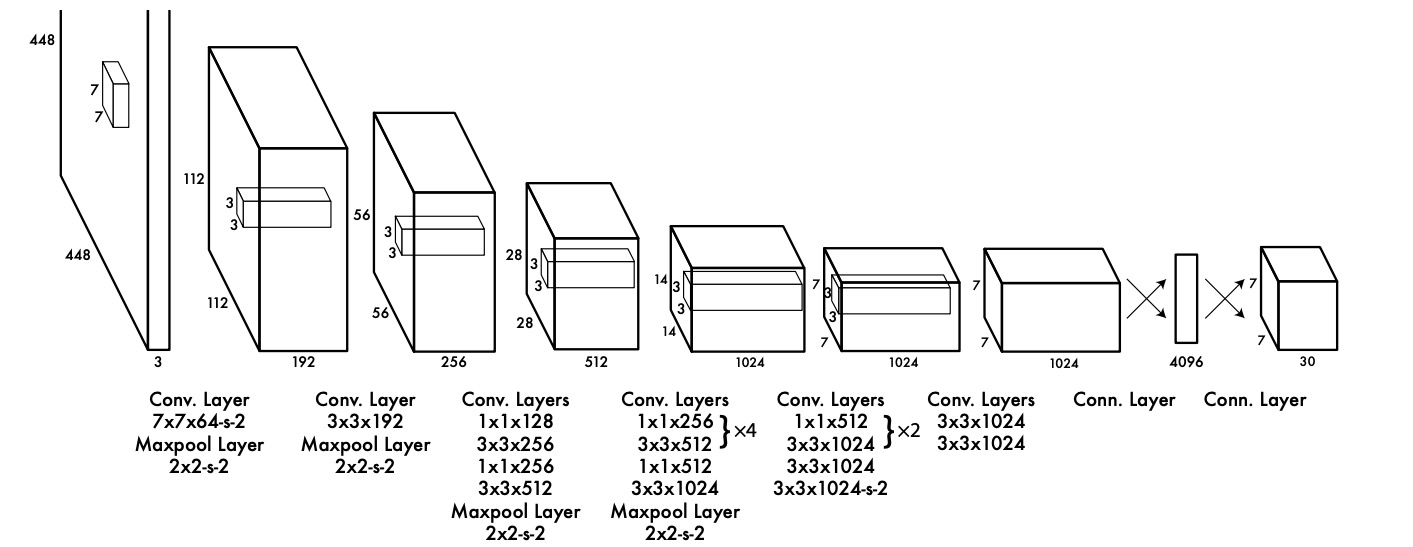
\includegraphics[scale=0.25]{CNN.jpg}
\caption{Convoluional Neural Network}
\label{fig:CNN}
\end{figure}

There are two main advantages of convolutional layers over fully connected layers, which are parameter sharing and sparsity of connections.

Parameter Sharing means a feature detector (such as a horizontal edge detector) that's useful in one part of the image is probably useful in all the other parts of the image. This is also true for higher level features, like detecting the curved body edge of snakes, and patterns on the body of snakes which can be used to distinguish categories of snakes. And being with a share the same parameters to compute all similar features, parameters are obviously reduced. Other than these, we don't need to learn separate feature detectors from scratch for our own neural network because the features of animals in images have some commonalities. Although some maybe look a little bit different by intuition, they are similar enough for computers after they are converted into pixels, and they can be detected by sharing feature detectors. That's why we can use transfer learning in computer vision tasks.

The second advantage is sparsity of connections. In the traditional neural network, since all neural units are connected, any unit of a layer is affected by all the units of the previous layer, and the effect of recognising an image is greatly reduced. In comparison, for convolutional layers, each region has its own unique features, and we do not want it to be affected by other regions, so we use convolution kernels (aka convolution matrix, or filter) to process a layer. In short, the rest of the pixel values other than the area we want to convolve do not have any effects on the output.

There are two types of pooling layers: max pooling and average pooling. For max pooling, it means we slide the filter through the input and take the largest element within the region covered by the filter. 
For average pooling, as the name suggests, it retains the average of the values encountered within the filter. pooling layers do not have any parameters to learn.

As for fully connected layer, it is a standard single layer of the neural network layer, where we have a matrix of weight and bias.

\subsection{Object Detection}

Object detection deals with detecting instances of objects of a certain class, such as humans, animals, etc, in digital images and videos. Object detection has applications in many areas of computer vision, including image retrieval, face detection, video surveillance, and self-driving, etc \cite{vedaldi2009multiple}. Current detection systems repurpose classifiers to perform detection. To detect an object, these systems take a classifier for that object and evaluate it at various locations and scales in a test image.

Object detection has made important progress in recent years. Mainstream algorithms are divided into two types: (1) two-stage detectors, such as R-CNN algorithm. The main idea is to adopt the heuristic method (selective search) first, or regional proposal network (RPN) to generate a series of sparse candidate boxes, and then classifies and returns these candidate boxes. This kind of approach needs two shots to detect objects, one for generating region proposals, one for detecting the object of each proposal. Such models reach the highest accuracy rate, but are typically slower \cite{he2017mask}; (2) single-stage detectors, such as YOLO (You Only Look Once) and SSD (Single Shot MultiBox Detector), that treat object detection as a simple regression problem by taking an input image and learning the class probabilities and bounding box coordinates. The main idea is to uniformly sample at different positions of the image. Different scales and aspect ratios can be used for sampling. Then, using convolutional neural networks to extract features and directly classify and return, the whole process only needs a single step, so its advantage is Fast. But an important disadvantage of uniform sampling is that the training is difficult, mainly because the positive and negative samples are extremely unbalanced, resulting in slightly lower model accuracy \cite{soviany2018optimizing}.

Considering that the object detection system needs to run on the iOS device, it needs to have a very high speed, so single-stage detectors have become our first choice, and I choose to implement YOLO for this project due to its excellent speed performance. YOLO came on the computer vision scene with the seminal 2015 paper “You Only Look Once: Unified, Real-Time Object Detection” by Joseph Redmon and immediately got a lot of attention by fellow computer vision researchers \cite{YOLO}. a TED talk was also made by Joseph Redmon from the University of Washington highlighting the state of the art in computer vision.

\begin{figure}[h]
\centering
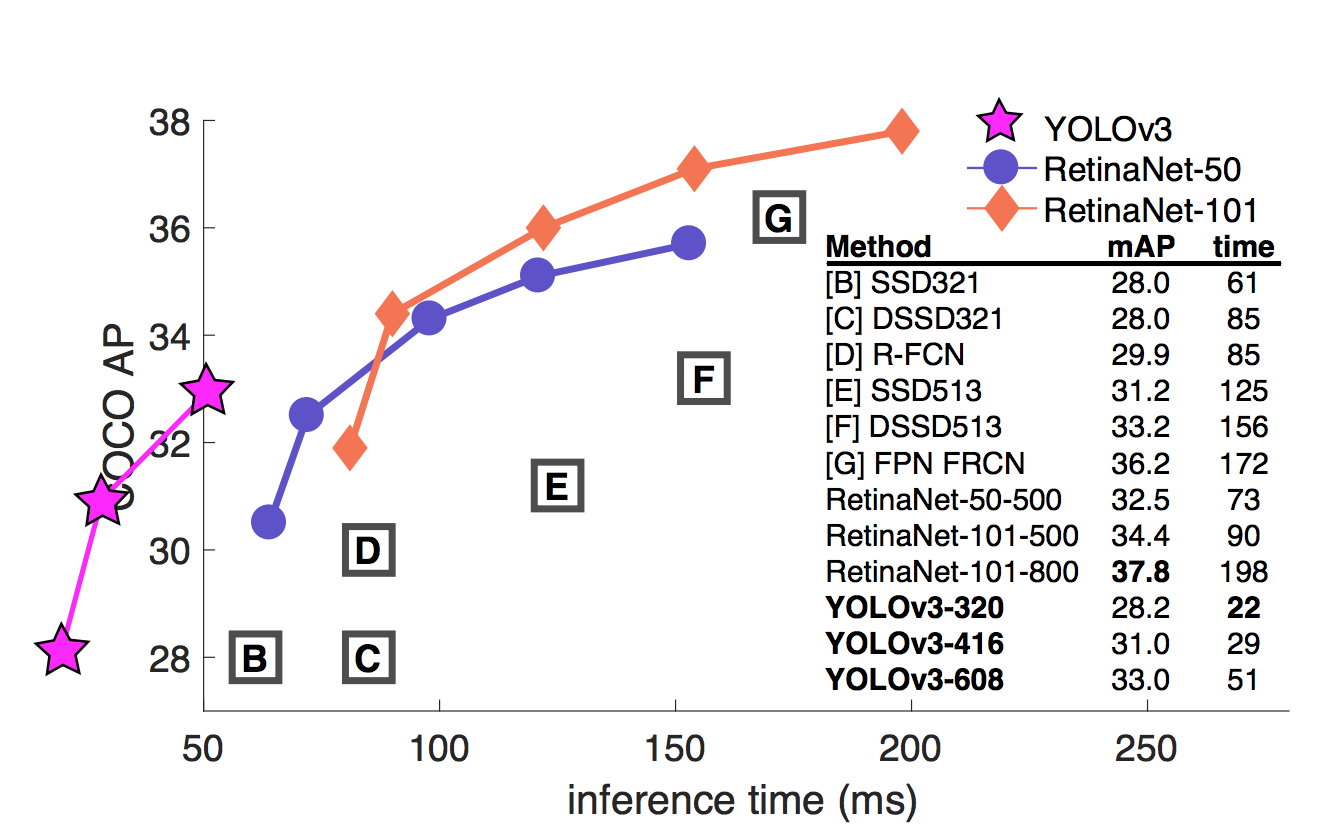
\includegraphics[scale=0.25]{YOLOv3.png}
\caption{Inference Time Comparison\cite{YOLO}}
\label{fig:YOLOv3}
\end{figure}


\textbf{Sliding Window}

Image detection is harder than image recognition because, in image detection, there can be multiple objects, or even maybe even multiple objects of different categories within a single image. At this time, sliding windows can help. We define a window of some size and put the window over a region on the image. Then feeding the input region to the convolutional neural network model to get an output. Likewise, we repeat this process on each and every region of the image with a certain stride \cite{lampert2008beyond}. Once done, we take a window of other sizes (longer, wider, etc) and slide the window over the image, and repeat this process again and again. We may probably end up with a window of the size of a snake in the image and seeing the model to output a breed for that window, meaning we detect a snake in that particular region.

\textbf{Bounding Box}

One of the disadvantages of sliding windows is the computational cost. As we crop out many square regions in the image, we run each region on a model independently. We may think of using a bigger window as it will reduce computation but, as a cost, the accuracy will decrease dramatically \cite{fowers2012performance}. Bounding boxes are the boxes that enclose the object in an image. The idea of bounding boxes is to divide the image into grids and then for each grid we define our Y label with some arguments. P is the probability that there is an object in the grid cell. If P equals to 0, then the other arguments are all ignored. Bx, By, Bh, Bw are respectively the x coordinate, the y coordinate, the height, the width of the bounding box. C1, C2... Cn refers to the class probability that the object is of a specific class. The number of classes may vary, depending on whether it’s a Binary Classification or Multi-Class Classification. If a grid contains an object, i.e. P equals to 1, then we know there is an object in a certain region of the image \cite{lempitsky2009image}. Now there are some issues we should consider, including how big is the size of the grid, which grid among all the girds whose P equals to 1 is responsible for outputting a bounding box for the object that span over multiple grids, etc. Usually, in practice 19 by 19 grid is used and the grid responsible for outputting the Bounding-Box for a particular object is the grid that contains the mid-point of the object. And, one more advantage of using 19 by 19 grid is that the chance of mid-point of the object appearing in two grid cells is smaller \cite{hillis2010bounding}.

\textbf{Intersection Over Union}

IOU means to divide the intersection of the bounding box and the true rectangle edge of the object by the union of them. The concept of intersection over union comes in to determine how accurate are these predictions. Suppose there are multiple bounding boxes an object in some grids, what intersection over union tells us is how close our prediction is to the ground truth. Then if the result is high enough (namely, greater than equal to a certain threshold) then the prediction is considered to be correct else we need to work on other bounding boxes \cite{ahmed2015optimizing}.

\begin{figure}[h]
\centering
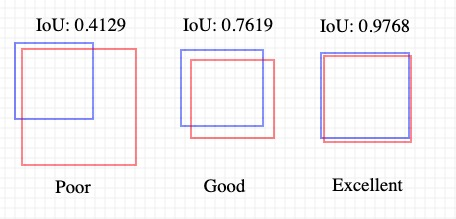
\includegraphics[scale=0.5]{IoU.jpeg}
\caption{Intersection over Union}
\label{fig:IoU}
\end{figure}

\textbf{Non-Max Suppression}

After doing intersection over union, for a prediction of a single object which spans over multiple grids, each grid would output its own prediction with a probability score, but it can make the predictions messy because there are multiple bounding boxes for a single object. What we do is, out of all the bounding boxes, we choose the box with the highest probability, and discard all the other boxes with a lower probability than the highest one. This is called non-max suppression.

\textbf{Anchor Box}

The last problem is how to detect multiple objects in the same grid cell. It is easy to deal with. The idea is to define multiple bounding box prediction values, that is to have many probabilities, x and y coordinates, heights, widths, and class confidences in a single array to refer to the class probability of an object, and this is called anchor boxes. 

\subsection{Framework}

There are many open-source deep learning frameworks gaining much popularity among researchers. I select Keras, using TensorFlow as backend, as the framework of this project.

Keras is a minimalist Python library for deep learning that can run on top of Theano or TensorFlow. It was developed to make implementing deep learning models as fast and as easy as possible for research and development. It is released under the permissive MIT license. It follows 4 guiding principles: (1) modularity: A model can be understood as a sequence or a graph alone. All the concerns of a deep learning model are discrete components that can be combined in arbitrary ways. (2) minimalism: The library provides just enough to achieve an outcome, no frills and maximizing readability. (3) extensibility: New components are intentionally easy to add and use within the framework, intended for researchers to trial and explore new ideas. (4) Python: No separate model files with custom file formats. Everything is native Python. TensorFlow is created by Google and used to replace Theano. The two libraries are in fact quite similar. Some of the creators of Theano. TensorFlow is written with a Python API over a C/C++ engine that makes it run faster. It is about more than deep learning and actually, it supports many algorithms to experience in other areas.

\subsection{iOS Application}

When facing large image recognition tasks, or using algorithms like R-CNN, it is hard for a mobile device to handle the task. At this time, maybe we can use internet transmission to transport the images to the server to finish the tasks. But in this project, since I use YOLO as the object detection algorithm, and the image captured by the camera is not too big, I choose to use CoreML and Vision as the development frameworks on iOS, and Swift as the development language.

CoreML is a brand new machine learning framework introduced by Apple at WWDC 2017. Unlike other open-source machine learning frameworks like PyTorch or TensorFlow, CoreML aims to help developers easily implement machine learning algorithms and build models, on iOS, macOS, watchOS, etc. CoreML lets developers integrate a broad variety of machine learning model types into their apps. In addition to supporting extensive deep learning with over 30 layer types, it also supports standard models such as tree ensembles, SVMs, and generalized linear models. Because it’s built on top of low-level technologies like Metal and Accelerate, CoreML seamlessly takes advantage of the CPU and GPU to provide maximum performance and efficiency.

Vision is a computer vision framework introduced by Apple at WWDC 2017 as part of Apple’s efforts to bring machine learning onto the iOS platform. Vision is a new, powerful, and easy-to-use framework that provides solutions to computer vision challenges. It is built on top of the CoreML framework and offers algorithms and utilities for working with computer vision tasks, such as face detection, QRcode recognition, etc. Before the Vision framework is imported, we may need to use some 3rd-party frameworks like OpenCV to achieve features. Generally, there are three steps to implement machine learning tasks on iOS: (1) loading the model. (2) creating the Vision request. (3) running CoreML.








\section{Object Detection}

\subsection{SSD}

SSD is a single-shot detector. It has no delegated region proposal network and predicts the boundary boxes and the classes directly from feature maps in one single pass. SSD speeds up the detecting process by eliminating the need of the region proposal network. To recover the drop in accuracy, SSD applies a few improvements including multi-scale features and default boxes. These improvements allow SSD to match the Faster R-CNN’s accuracy using lower resolution images, which further pushes the speed higher. It achieves the real-time processing speed and even beats the accuracy of the Faster R-CNN. 

The SSD object detection composes of 2 parts: (1) extract feature maps, (2) apply convolution kernels to detect objects. SSD uses VGG16 to extract feature maps. Then it detects objects using the next layer. Each prediction composes of a boundary box and 21 scores for each class, and we can pick the highest confidence as the class for the object. To improve accuracy, SSD introduces: (1) small convolutional filters to predict object classes and offsets to default boundary boxes. (2) separate filters for default boxes to handle the difference in aspect ratios. (3) multi-scale feature maps for object detection \cite{liu2016ssd}.

Besides, SSD can be trained end-to-end for better accuracy. SSD makes more reduction and has better coverage on location, scale and aspect ratios. With the improvements above, SSD can lower the input image resolution to 300 * 300 with a comparative accuracy performance. By removing the delegated region proposal and using lower resolution images, the model can run at real-time speed and still beats the accuracy of the state-of-the-art Faster R-CNN.

\begin{figure}[h]
\centering
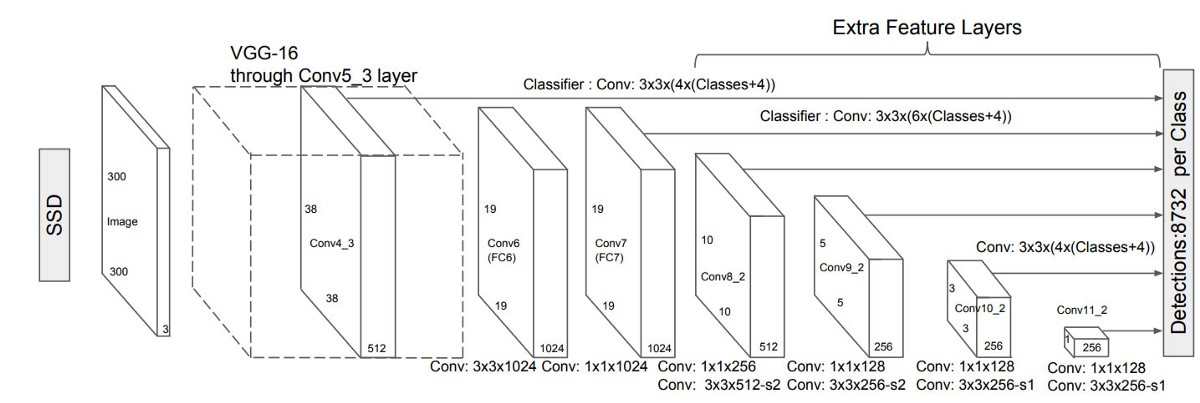
\includegraphics[scale=0.25]{SSD.jpeg}
\caption{SSD\cite{liu2016ssd}}
\label{fig:SSD}
\end{figure}

\subsection{YOLO}

YOLO stands for "You only look once". It is refreshingly simple, and it uses a single convolutional network simultaneously predicts multiple bounding boxes and class probabilities for those boxes. YOLO trains on full images and directly optimizes detection performance. This unified model has several benefits over traditional methods of object detection: extremely fast, and achieves more than twice the mean average precision of other real-time systems \cite{YOLO}.

\subsection{YOLO9000}

The problem with YOLO is that it is not accurate enough. It has a higher error rate in target positioning than Fast R-CNN. Therefore, improvements to YOLO focus on enhancing positioning accuracy while maintaining classification accuracy. The approaches include batch normalization, using high-resolution images, convolving with anchor boxes, dimension clusters, direct location prediction, fine-grained features, and multi-scale training \cite{YOLO9000}.

\begin{figure}[h]
\centering
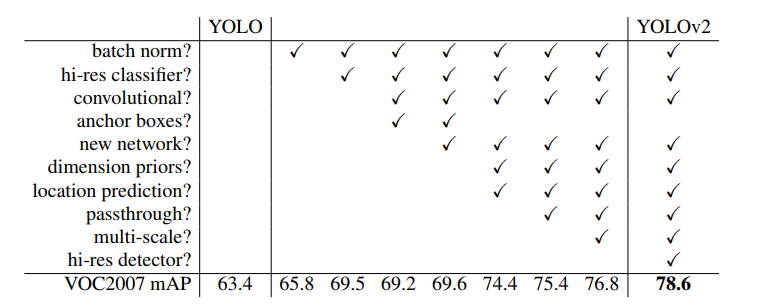
\includegraphics[scale=0.6]{YOLOv2.PNG}
\caption{YOLO9000\cite{YOLO9000}}
\label{fig:YOLO9000}
\end{figure}

Firstly, batch normalization can increase the speed of model convergence and reduce overfitting. In YOLO9000, Batch Normalization is applied to all convolutional layers, which increases the result by 2\% mAP. At the same time, the application of Batch Normalization removes the dropout without overfitting. Secondly, high-resolution images are adapted to the network, then the network was used for the target detection task finetune. High-resolution images increase the result by 4\% mAP. Thirdly, the fully connected layers are abandoned and anchor boxes are used to predict bounding boxes. Before it predicts 98 boxes per image with fully connected layers, but with anchor boxes, each image can predict more than 1000 boxes. Although the mAP dropped after using anchor boxes, the recall increases by 7\%. Fourthly,  YOLO9000 uses k-means clustering which leads to good IOU scores, and k = 5 is the best value with a good tradeoff between model complexity and high recall. Fifthly, the predicted offset is changed to the position coordinate of the predicted grid cell, and the predicted value is limited to the range of 0-1 to enhance stability. Sixthly, adding a passthrough layer to the network to add features. Passthrough is similar to ResNet, combining high-resolution features with low-resolution features to convert a 26 * 26 * 512 feature map into a 13 * 13 * 2048 feature map, which improves the performance by 1\%. Finally, and the most important, The model input size is changed every few batches to make the model more robust to different-size images. Every a few batches, the model randomly selects a new input image size to change the model input size, and continues training. This rule forces the model to adapt to different input resolutions \cite{YOLO9000}.

\subsection{YOLOv3}

The main differences between YOLOv3 and YOLO9000 are as follows. First, YOLO v3 uses a variant of Darknet, which originally has 53 layer network trained on Imagenet. For the task of detection, 53 more layers are stacked onto it, giving us a 106 layer fully convolutional underlying architecture for YOLO v3 \cite{YOLOv3}. Then, The most salient feature of v3 is that it makes detections at three different scales, and the detection is done by applying 1 * 1 detection kernels on feature maps of three different sizes at three different places in the network. Thirdly, for an input image of the same size, YOLOv3 performs more bounding boxes than YOLO9000 on it. Besides, the squared loss function in YOLO9000 is replaced by cross-entropy loss function in YOLO v3, they’ve been replaced by cross-entropy error terms. In other words, object confidence and class predictions in YOLO v3 are now predicted through logistic regression. Finally, YOLOv3 performs multilabel classification for objects detected in images \cite{YOLOv3}.

YOLOv3's COCO AP metric is on par with SSD but 3x faster. In particular, its IoU equals to 0.75, which drops significantly comparing with RetinaNet which suggests YOLOv3 has higher localization error. YOLOv3 also shows significant improvement in detecting small objects.

\begin{figure}[h]
\centering
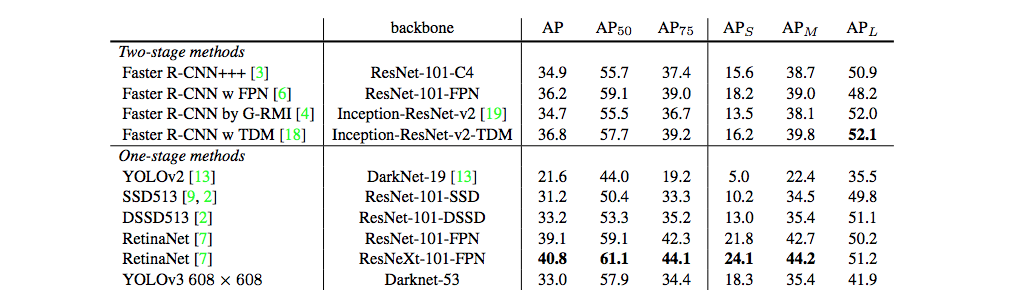
\includegraphics[scale=0.4]{COCO.png}
\caption{COCO AP\cite{YOLOv3}}
\label{fig:COCO AP}
\end{figure}










\section{Data set}

For the majority of computer vision problems, the quality and quantity of the dataset determine the performance of the neural network to a large extent. All the images will be transferred into the same-resolution pixels for the purpose to be recognized and distinguished by computers, then fed into the neural network, used to train the model in many epochs, and finally, after being convolved and pooled, become a confidence matrix, which is the output of the neural network.

For quality, it means that good datasets should include an object (sometimes may be multiple objects) to be classified, high resolution, exact label and bounding box information (only for object detection). For quantity, however, the image classification problem requires a huge amount of data which is extremely difficult to obtain. Thus collecting data becomes the most difficult part of all the jobs.

The number of breeds of snakes in Australia is roughly estimated at more than 30. Most of the breeds are covered in this project but not all, since some of which are rare and the images of these species are extremely hard to obtain. Every image is carefully censored and labelled before putting into the dataset.

\subsection{Data Retrieving}
In order to collect data, lots of data sources are tried but only a few are utilized given their quality of images. The most source used to collect data is Google Image. For each breed of snakes, batches of images can be retrieved by searching the breed name, and then the search results can be downloaded in bulk through Python scripts.

ImageNet is a large visual database designed for computer vision research. It contains more than 14 million images and more than 20,000 categories with a typical category. What is most impressing is that each image has bounding box information, which is wonderful for training model for object detection. Depressingly, The top search results under "snake" on ImageNet are Cobra, Night Snake, King Snake, etc., but for this project, we are focusing on snakes in Australia, none of which exists on ImageNet.

There are also some other datasets used in this project, including the Australian Reptile Online Database, Science Photo Library, The Reptile Database. However, the quality of these databases is quite low compared to Google Image, and the quantity is relatively small. Also, there are other problems existing on these databases, like wrongly-labelled.

\subsection{Data Preprocessing}
Although a huge amount of data are gathered, not every single image satisfy the requirement for being fed into neural networks. Also, for coloured images with three channels, we cannot put them into the neural network directly just like how grayscale images are dealt with. Therefore data preprocessing is needed to ensure the compliance of data from different sources, and also to enhance the performance of the model.

(1) The first thing is to filter out low-resolution images. In this project, the scale of images fed into the neural network should be larger than 224*224 (width * height) pixels, otherwise, it will throw out the error that the image does not fit the input of the model. We can do some image stretching or interpolation to expand the scale of an image to the suitable size, but it just uses the pixel information already exist in the original image, which is useless for improving the accuracy of the model.

<image/low resolution>

(2) The second kind of images should be handled is that the images with much redundant information, especially for images with background occupying a large area and images with some unrelated objects in it. The proportion of the needed object (here the snake) should take most of the area and cannot be overwhelmed by information with no benefit to the results. To avoid this situation, clipping is a good approach to get rid of redundant information.

<image/redundant objects>

<image/without enough information>

(3) Some images downloaded from the Internet lack the label or are wrong-labelled. We must manually inspect each of the images and give those images the right label by examing and comparing them with the right breed of each.

(4) Before feeding the images into the neural network, all input images need to be reshaped to a certain scale (224*224 pixels in this project) to ensure the input layers can convolve the images correctly. The resize function in the OpenCV library is effective to handle this problem.

(5) Image normalization is an important step which ensures that each input pixel has a similar data distribution to facilitate the robustness of training. Image normalization transforms the raw images into a unified form, gets rid of innate structure inside the dataset by perturbing images, and makes it faster for training to converge. There are many ways to do image normalization, including Min-max Normalization and Zero-mean Normalization, etc. Min-max Normalization is done by subtracting the minimum value of all pixels and then dividing by the maximum value minus the minimum value of all pixels. Zero-mean Normalization is done by subtracting the mean of every pixel and then dividing by the standard deviation of every pixel where the first step aims to keep the sum of all values of the three channels equal to zero and the second step aims to make the variance of the values of the three channels equal to one. The process of normalization is essential for most deep learning tasks other than only computer vision problems. In this project, image normalization is accomplished by using the scale function in the preprocessing module of the sklearn library.

\subsection{Data Augmentation}
When training computer vision models, collecting more data is an effective way to enhance the training but also a tedious and intricate process. In fact, for the majority of image recognition problems, we cannot get as much data as we expect. In order to obtain more data, data augmentation techniques is a very efficient method to improve the result.

Data augmentation contains many methods, including flipping, rotating, cropping, scaling, warping, color shifting, adding noise, etc.

Also there are different ways to do data augmentation. One is offline augmentation, which means to perform all augmentations in advance before starting to build the neural network, and store all the images on hard disk drivers. It can access data very fast once after images are loaded into the memory, but it will increase, or multiple, the size of the dataset, which consumes memory to a large extent, so this method fits small datasets well. The other one is online augmentation, which means to perform the augmentation on a mini-batch dataset right before they are fed into the neural network. This method is more suitable for large datasets because the memory is limited for staging large scale images. For this project, the total number of images we have is which is not big, so both methods are fine. For offline augmentation, we can use the imgaug library which has powerful stochastic interface to augment images, and, for online augmentation, we can use the ImageDataGenerator function in the preprocessing.image module in Keras.

\subsection{Dataset Split}









\section{Training}

\subsection{Callback Function}

\subsection{Dropout}

\begin{figure}[h]
\centering
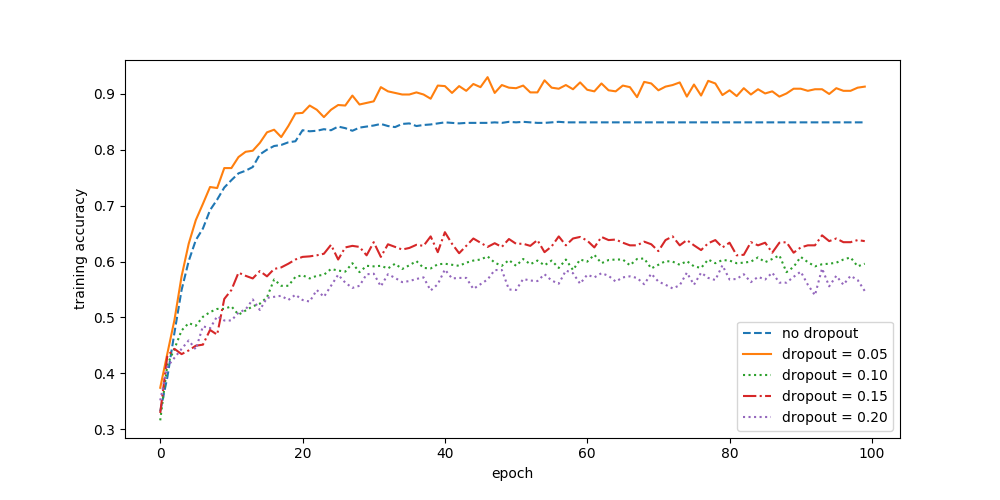
\includegraphics[scale=0.5]{DataAnalysis/TrainingAccuracyDropout.png}
\caption{Training Accuracy with Different Dropout}
\label{fig:Training Accuracy with Different Dropout}
\end{figure}


\begin{figure}[h]
\centering
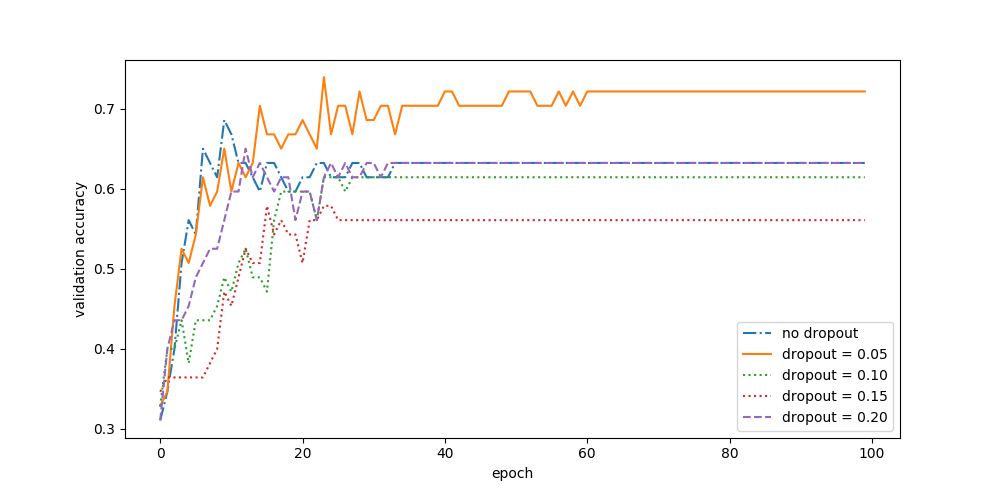
\includegraphics[scale=0.5]{DataAnalysis/ValidationAccuracyDropout.png}
\caption{Validation Accuracy with Different Dropout}
\label{fig:Validation Accuracy with Different Dropout}
\end{figure}

\subsection{Neural Units}


\begin{figure}[h]
\centering
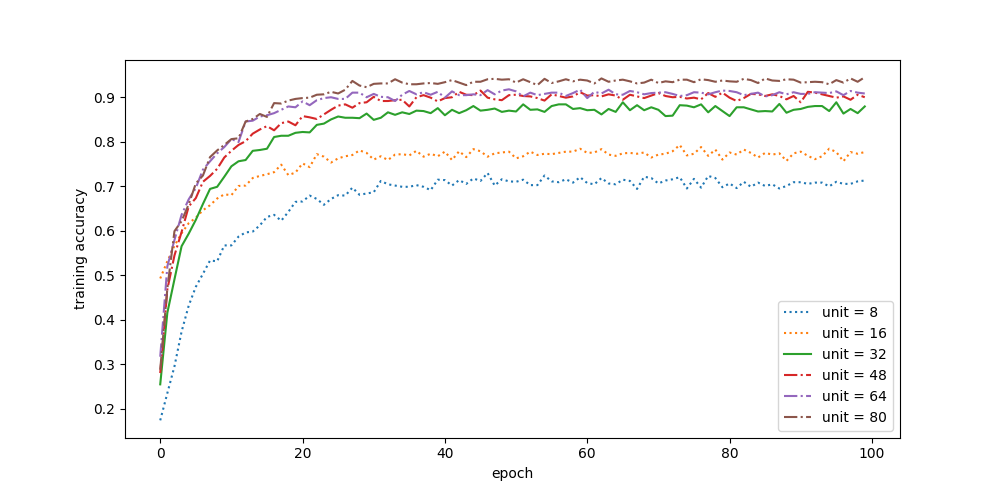
\includegraphics[scale=0.5]{DataAnalysis/TrainingAccuracyUnit.png}
\caption{Training Accuracy with Different Unit}
\label{fig:Training Accuracy with Different Unit}
\end{figure}

\begin{figure}[h]
\centering
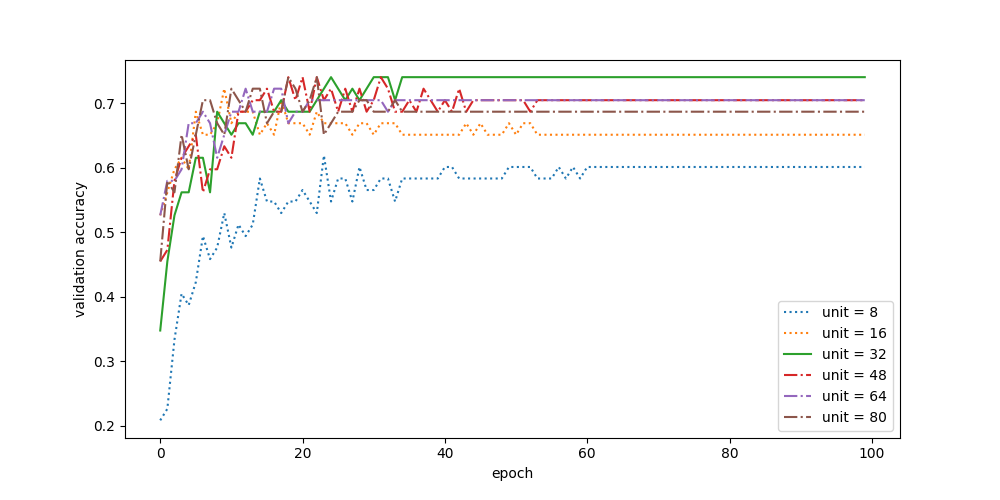
\includegraphics[scale=0.5]{DataAnalysis/ValidationAccuracyUnit.png}
\caption{Validation Accuracy with Different Unit}
\label{fig:Validation Accuracy with Different Unit}
\end{figure}










\section{iOS Application}

\subsection{Design}

The iOS application contains 5 view pages. One is the main view page, which is responsible for showing names of all kinds of snakes, with two buttons at the bottom for users to enter the object detection view page and the image capture view page. The object detection view page is only for detecting snakes. The image capture view page is for capturing images. You can flip the camera to use the front and the back camera. Also, you can pick one photo in the Photos library of your iPhone. When you press the capture button or choose one photo from the Photos library, you will enter a breed identification view page. This identification view page is just for transition, and to indicate that the phone is processing the image. At last, after identifying the image, you will enter an information view page, showing the type, venom, area, and the description of the snake you just captured. If the confidence is below a certain value, the app considers that what you captured is not a snake in Australian, and makes a relevant prompt.

\begin{figure}[h]
\centering
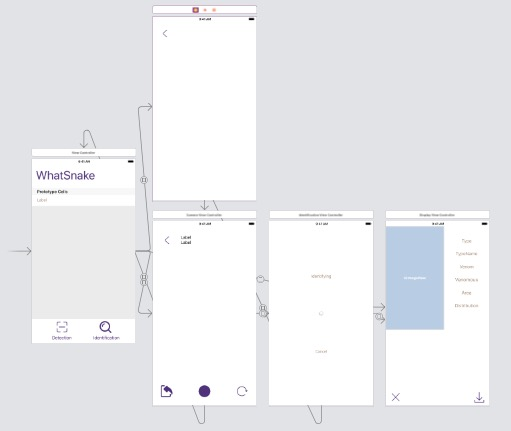
\includegraphics[scale=0.7]{viewpage.jpg}
\caption{View Pages}
\label{fig:viewpage}
\end{figure}

\subsection{YOLOv3 on iOS}

With the principle of implementation of YOLOv3 in mind, we can build the pipeline of Object Detection on iOS from scratch step by step. There are some important parameters in the implementation of YOLOv3 algorithm, including the input image width, the input image height, the max number of bounding boxes, the IOU value and its threshold, the confidence of each class in the prediction and the threshold of confidence. For the bounding boxes, the built-in class of CAShapeLayer and CATextLayer are used to represent the bounding boxes and to compute the confidence of whether there is an object within the bounding boxes.

This part of codes is under the folder YOLOv3 in the iOS folder.

\subsection{Implementation}

\textbf{Camera}

In order to use the camera, we should first create a new view controller (usually named CameraViewController) and import the library UIKit and AVFoundation. Then place a button preview layer on the view controller. the AVFoundation variables are needed to operate on the camera, including AVCaptureSession to enable the capture session, AVCaptureDevice to enable the front and the back camera, AVCapturePhotoOutput to capture a photo to be transited to another view controller. Then start configuring the camera in the viewDidLoad method. Making the preview layer fit the view controller is important. Finally, what we need to do is to run the app on a real device because the simulator doesn’t have a camera, so it won’t actually run.

\textbf{Recognition}

VNCoreMLRequest is an image analysis request that uses a CoreML model to process images. The results array of a CoreML-based image analysis request contains different observation types. In order to let the image captured by the camera be recognized by the model, we can simply create an instance of VNCoreMLRequest and use DispatchQueue.main.async to process the image asynchronously without user operation blocked.

\textbf{Transmission Objects}

View controllers (more precisely, UIViewController) are the basic component units in organizing an iOS application. Each view controller has its own class. The interaction operations between view controllers in Cocoa Touch Class have already been encapsulated, so it's not possible to transmit objects using return in functions as usual. There is a function called "prepare" in the UIViewController class, which is used to transmit object between view controllers using a pipeline called "segue". We can override this prepare function, designating the "for segue" argument to specify which segue and view controllers we want to operate, in order to finish the transmission.

\section{Conclusion}

\section{Future Work}

\bibliographystyle{plain}
\bibliography{references}
\end{document}


% \begin{figure}[h!]
% \centering
% \includegraphics[scale=1.7]{universe}
% \caption{The Universe}
% \label{fig:universe}
% \end{figure}
